Após desenvolver os métodos descritos nas seções \ref{sec:genetico} e \ref{sec:simplex} como funções do MATLAB, foram feitas algumas alterações na interface desenvolvida anteriormente \cite{trabalho2} para englobar esses novos métodos, conforme ilustrado na figura \ref{fig:gui}\\

\begin{figure}[H]
	\begin{center}
		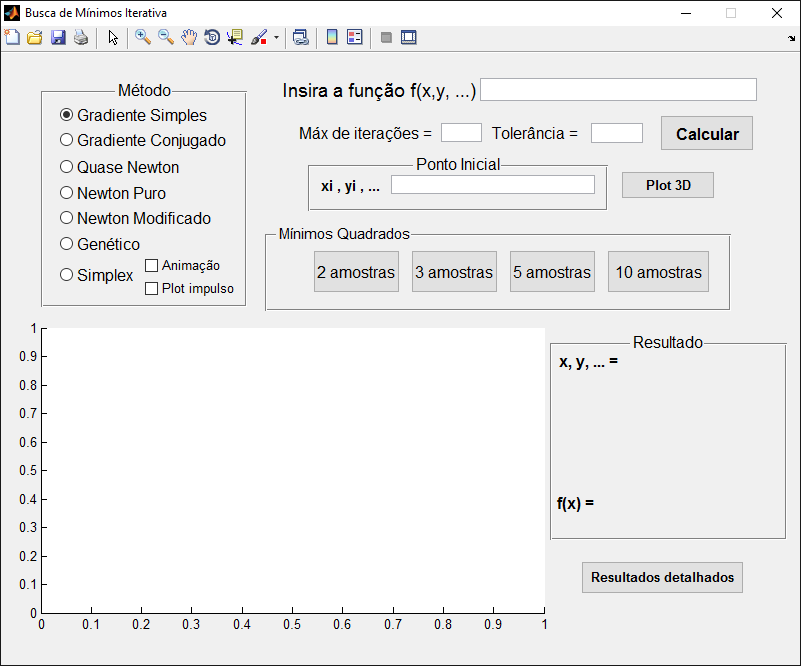
\includegraphics[width=16cm]{GUIfinal}   
		\caption{Janela do programa de Busca de Mínimos Iterativa.}
		\label{fig:gui}
	\end{center}
\end{figure}

\par Há um grupo de 4 novos botões, que servem para a resolução do problema de mínimos quadrados apresentado nesse trabalho. Ao clicar em um desses botões, a função de erro quadrático com 2, 3, 5 ou 10 amostras é automaticamente colocada na caixa de texto \textit{Insira a função f(x,y,...)}. Assim, o usuário pode facilmente tentar encontrar os parâmetros desejados da função de transferência, testando para os diferentes métodos implementados.\\

\par Na aba \textit{Método} houve a adição das 2 novas funções, e o método simplex também apresenta dois parâmetros extras. Ao marcar a opção \textit{Animação}, o programa mostra cada passo da minimização pelo algoritmo simplex e o usuário consegue ver bem cada etapa do processo, passando para a próxima com um clique do mouse ou pressionando qualquer tecla (incluindo efeitos sonoros). Já a opção \textit{Plot Impulso} serve para quando a função de mínimos quadrados for a função minimizada, assim que o mínimo for encontrado, o programa mostra um gráfico da resposta ao impulso do sistema proposto nesse trabalho, com os coeficientes que acabaram de ser calculados.
